\documentclass[a4paper, titlepage, twocolumn, 10pt]{article}
\usepackage{amsmath, gensymb, graphicx, float}
\usepackage{listings}
\title{\textbf{ECSE 307 Linear Systems and Control} \linebreak Lab 4 Assignment}
\author{Xu HAI, 260661832 \and Wenjie WEI, 260685967}
\date{October 27$^{th}$, 2017}
\usepackage{color} %red, green, blue, yellow, cyan, magenta, black, white
\usepackage{inconsolata}
\definecolor{mygreen}{RGB}{28,172,0} % color values Red, Green, Blue
\definecolor{mylilas}{RGB}{170,55,241}


\lstset{language=Matlab,%
	%basicstyle=\color{red},
	basicstyle=\ttfamily,
	breaklines=true,%
	morekeywords={matlab2tikz},
	keywordstyle=\color{blue},%
	morekeywords=[2]{1}, keywordstyle=[2]{\color{black}},
	identifierstyle=\color{black},%
	stringstyle=\color{mylilas},
	commentstyle=\color{mygreen},%
	showstringspaces=false,%without this there will be a symbol in the places where there is a space
	numbers=left,%
	numberstyle={\tiny \color{black}},% size of the numbers
	numbersep=9pt, % this defines how far the numbers are from the text
	emph=[1]{for,end,break},emphstyle=[1]\color{red}, %some words to emphasise
	%emph=[2]{word1,word2}, emphstyle=[2]{style},    
}

%Main content
\begin{document}
	\maketitle
	% Make the title
	\newpage
	\pagenumbering{gobble}
	% Remove the page number
	
	% ===================================================
	% Question 1
	% ===================================================
	
    \section{Problem 1}
	For this question, we are exploring something about the equation below.
	\begin{align}
	G(s)=\frac{1}{(s+1)(s+2)(s+3)} \label{limit}
	\end{align}
	\subsection{Draw the step response of the function}
	Since we know $(s+1)(s+2)(s+3) = x^3 + 6x^2 + 11x + 6$. To find the step response, the following MATLAB code is implemented.
	\begin{lstlisting}[frame=single]
G = tf([1], [1, 6, 11, 6]);
step(G);
	\end{lstlisting}
	The graph is shown as follow:
	\begin{figure}[H]
		\centering
		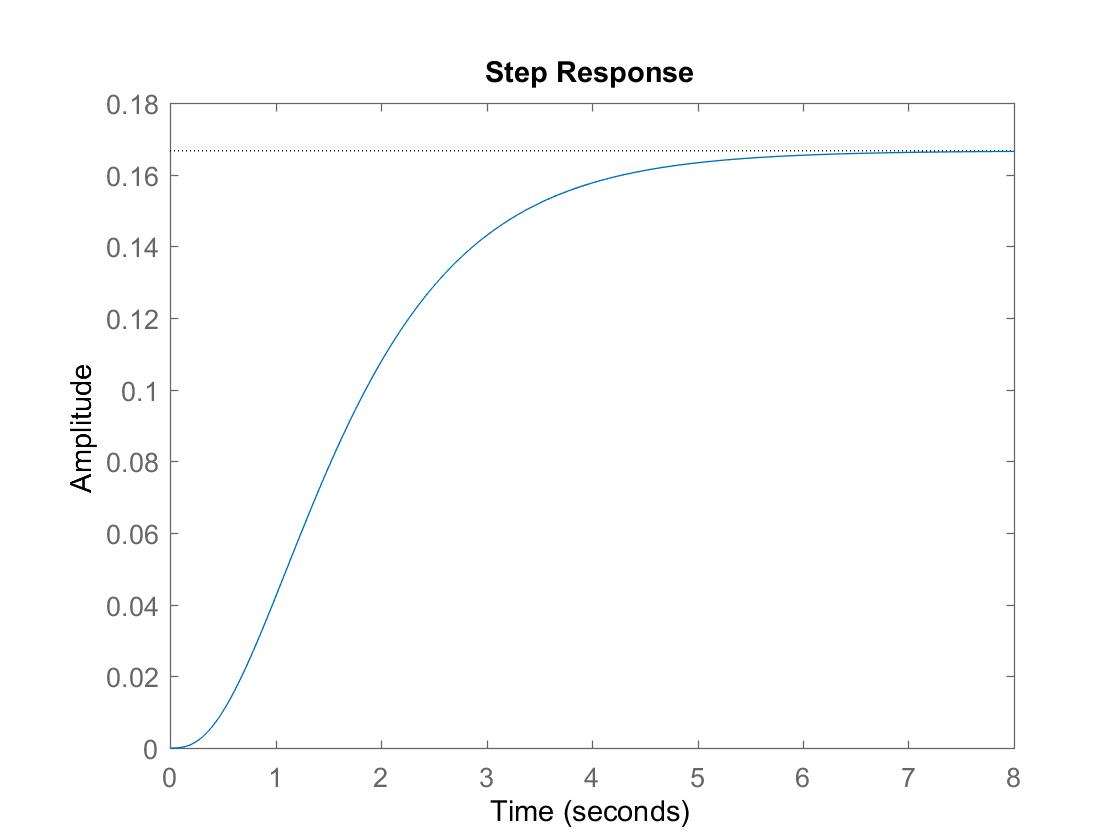
\includegraphics[width=0.5\textwidth]{1-a}
		\caption{The step response of the function}
		\label{1-a}
	\end{figure}

	\subsection{The step function information of this system}
	
	\subsection{Values for the steady state error, rise time, settling time and overshoot}
	
	\subsection{Root locus of the open loop system}
	
	\subsection{The gain and the frequency of at the marginal stability}
	
	\subsection{The proportional controller}
	Using the following code, we can add the proportional controller.
	\begin{lstlisting}[frame=single]
C_P = pid(40);
open_loop = series(C_P, G);
H1 = feedback(open_loop, 1);
hold on;
figure;
step(H1);
stepinfo(H1);
	\end{lstlisting}
	\subsection{The drawbacks and benefits of using proportional controller}
	
	\subsection{The derivative controller}
	Using the following code, we can add the derivative controller.
	\begin{lstlisting}[frame=single]
C_PD = pid(40, 0, 30);
open_loop_PD = series(C_PD, G);
H2 = feedback(open_loop_PD, 1);
hold on;
figure;
step(H2);
stepinfo(H2);
	\end{lstlisting}
	\subsection{The characteristics can be improved and the benefits of adding derivative controller}
	
	\subsection{Keep the proportional controller and add the integral controller}
	Using the following code, we can keep the proportional controller and add the integral controller.
\begin{lstlisting}[frame=single]
C_PD = pid(40, 10, 0);
open_loop_PD = series(C_PI, G);
H3 = feedback(open_loop_PI, 1);
hold on;
figure;
step(H3);
stepinfo(H3);
\end{lstlisting}	
	\subsection{The characteristics can be improved and the benefits of adding integral controller}
	
	\subsection{Analysis about Kp}
	
	\subsection{PID controller}
	Using the following code, we can use P, I and D controller together.
\begin{lstlisting}[frame=single]
C_PD = pid(19, 12, 8);
open_loop_PD = series(C_PID, G);
H5 = feedback(open_loop_PID, 1);
hold on;
figure;
step(H5);
stepinfo(H5);
\end{lstlisting}

% ========================================================
% Question 2
% ========================================================

	\section{Problem 2}	
	
\end{document}
